\section{Freshness Scheduling}
Process execution parameters are set by the user when a process element is created.  Generally, job scheduling is strictly driven
by these parameters.  However, in our deployments we found there were job pipe sinks that required a \emph{minimum freshness}
property for the set of data points in the buffer upon consumption.  In this section we discuss our scheduling algorithm in
relation to providing this property.% and present some experimental results.


\subsection{Maximizing Data Freshness}
\label{sec:freshness}

Data is coming in at different, independent rate from sensors and is produced asynchronously from internal processing elements.
For certain processes, the freshest
data from all the streams they are subscribing to is necessary; while minimizing the average time that the data for each respective 
stream has 
been waiting in the buffer.


\begin{algorithm}[h!]
 \SetAlgoLined
 Given a full buffer $b[n]$:\\
  \For{all elements in the $b$}{
  (1) Calculate the staleness of element $i$ and add to total staleness, $S_n$\;
  \For{all other elements in the buffer}{
    (1) Determine the next report time $D_i$ for this element\;
    (2) Determine the staleness of all the elements if we wait until $D_i$\;
    (3) If it is the smallest staleness figure calculate, replace minimum cost, $S_l$.
    }
  }
  \If{$S_l$ is less than $S_n$}{
  (1) Wait until later to consume\;
  \Else{
  (1) Consume now}
  }
 \caption{\texttt{min\_buffer} algorithm.}
 \label{alg:min_buffer}
\end{algorithm}

Some streams show lots of variability, driven by the underlying dynamics of the system being monitored.  For example, the power
consumption of an active server or laptop tends to have a very active power profile.  For jobs doing aggregation of 
streaming data, it is often the case that the time when the last reading was received is very different across streams.  
For example, consider two rapidly changing streams.  The ideal aggregation scenario is to
combine the streams from the latest readings for both streams.  That way you minimizing the offset difference between during aggregation.
If stream 1 produces a reading every 3 seconds and stream 2 produces a reading every 2 seconds, and you aggregate the readings every time you
have at least one reading from both streams, every 3 seconds.  Sometimes the reading from the 2-second stream will be 1 second old.
If run the computation \emph{now}, the total staleness of the buffer is 1 second, if we wait on more second the total staleness is still 1 second, because
at t=4 seconds, the 3-second stream will be 1 second old.
For applications that wish to display the freshest aggregates with the latest results (smallest buffer staleness), we provide an algorithm
called \texttt{min\_buffer}.

Certain jobs only care about consuming the latest readings from their subscription streams.  They are willing to discard reading until two
conditions are met:

\begin{enumerate}
\item There is at least one data point from each stream in the subscription buffer.
\item The staleness factor is minimized within the immediate time window.
\end{enumerate}

% This is of particular interest to controllers that need to make control decision based on the freshest data possible and can tolerate some variability
% in the completion time of the control task.  It is also useful in analytical jobs that want to process the latest data from multiple streams while also
% allowing some variability in the completion of the processing task.  
Note, there's a fundamental tradeoff
between the staleness factor and variability of consumption.  It is sometimes better to wait for the next incoming data point than it is to use what
is currently in the buffer, as waiting will decrease the overall staleness factor.  Other times, it is better to consume the buffered data immediately.
This causes a certain amount of variability in the delivery period to the control process.  However, for some applications, this is a reasonable tradeoff
to make.  Making use of the freshest data is desirable for minimizing errors, either in the control of a system or the calculation of some aggregate 
state.
Generally, the error grows with staleness, therefore the goal of this mechanism is to continuously minimize the error associated with staleness through
scheduling.


\begin{figure}[t!] %htbp
\centering
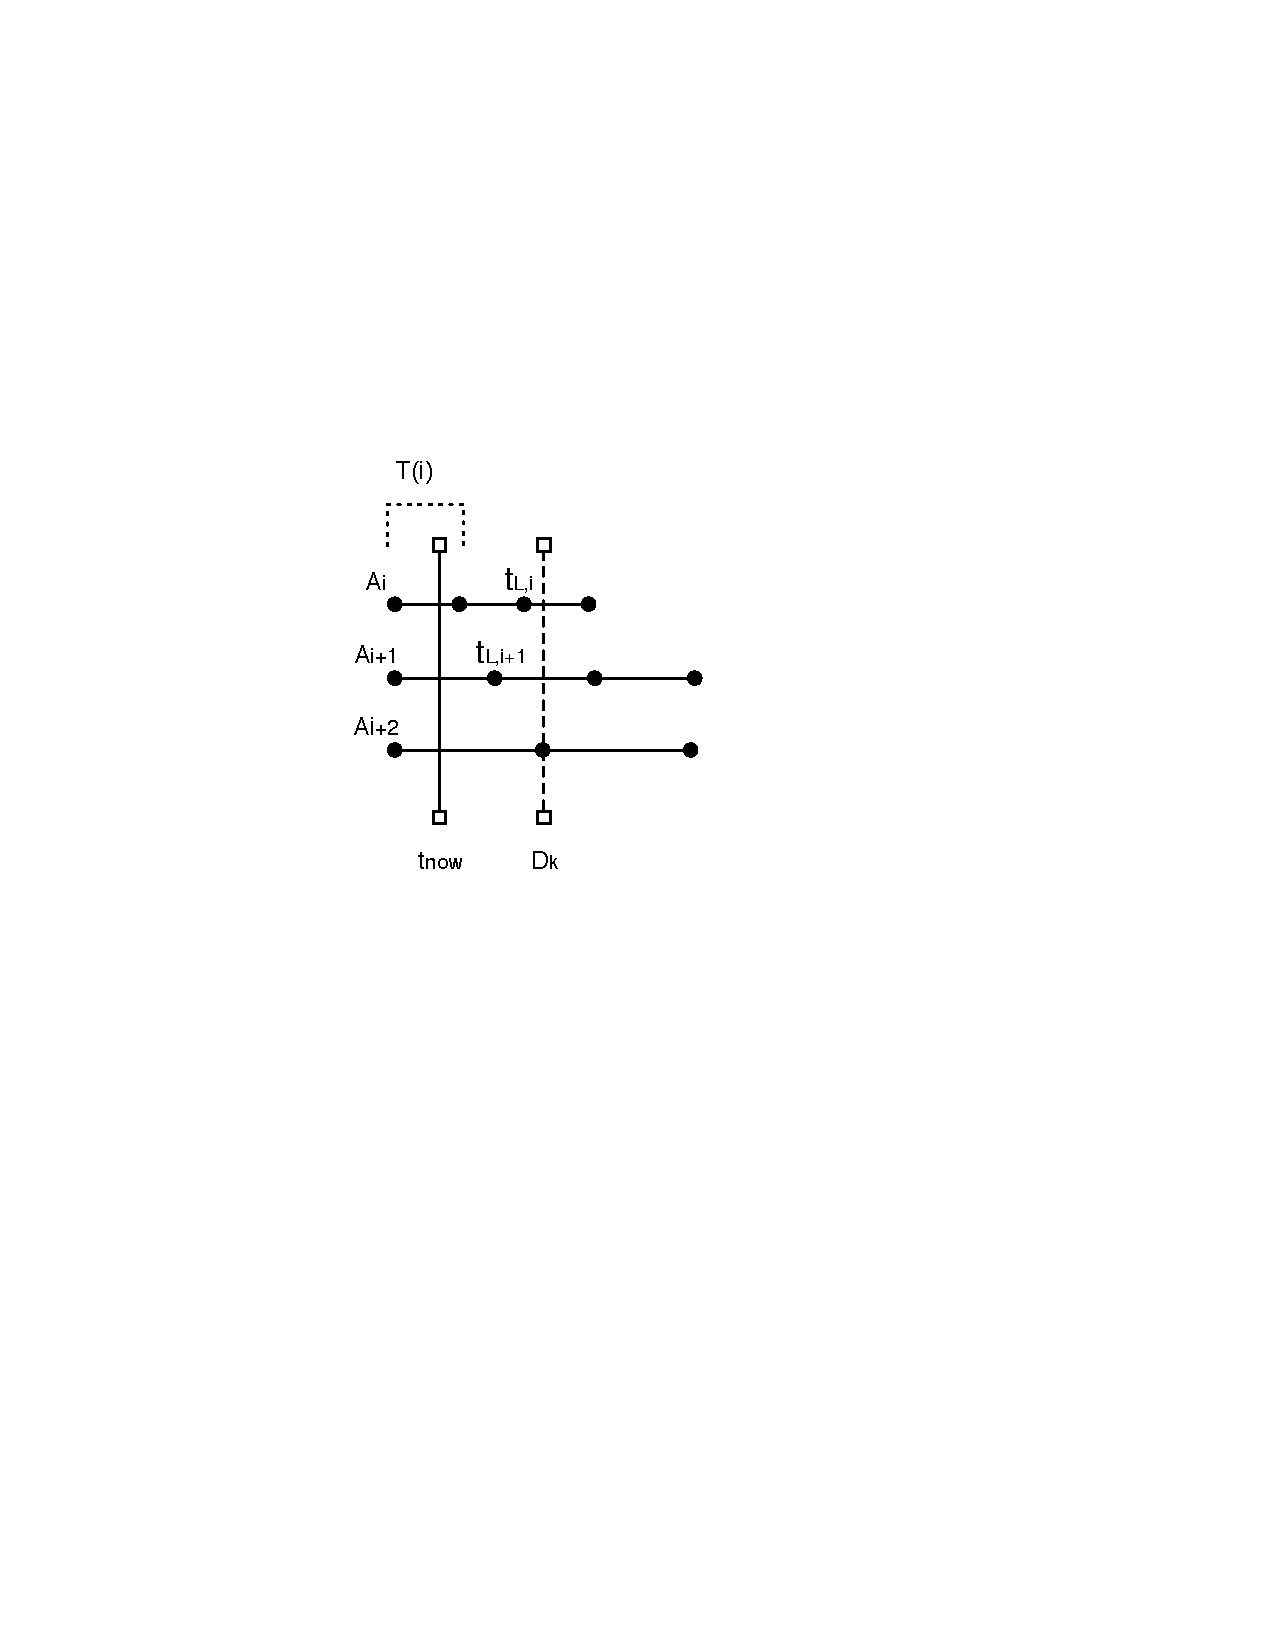
\includegraphics[width=0.75\columnwidth]{figs/min_buffer}
\caption{Multiple streams in a subscription and their associated parameters.}
\label{fig:min_buffer}
\end{figure}

Let $A_{i}$ be the arrival time of the last data point received from stream $i$ and $D_{i}$ be the arrival time for the next data point from stream $i$
and their relationship as described in equation \ref{eqn:deadline}, where $T(i)$ is the average period between the arrivals from stream $i$.

\begin{equation}
D_{i} = A_{i} + T(i)
\label{eqn:deadline}
\end{equation}


Periodically, our algorithm runs and checks if there is a data point for each stream in the subscription.  If so, the \emph{min\_buffer} algorithm runs 
and effectively decides whether to execute the job on the current buffer immediately or whether to wait until later, when the \emph{staleness factor} of
the buffer will be at a minimum.  This decision is driven by equation~\ref{eqn:later_better_condition}, whereby we find the next deadline, computed with
equation~\ref{eqn:last_deadline}, for each stream in the set and determine the staleness factor will be for the entire buffer if we wait until that deadline arrives.

\begin{equation}
t_{L,i} = A_{i} + \Bigl\lfloor \frac{D_{k}-A_{i}}{T(i)} \Bigr\rfloor T(i)
\label{eqn:last_deadline}
\end{equation}

If there is no deadline $D_{k}$ for some stream $k$ such that equation~\ref{eqn:later_better_condition} holds, then we execute now.  Otherwise we choose to wait
until $D_{k}$ for the stream whose next deadline minimizes the staleness factor of the buffer.


\begin{equation}
\sum_{i=1}^{k-1} D_{k} - t_{L,i} < \sum_{i=1}^{k} t_{now} - A_{i}
\label{eqn:later_better_condition}
\end{equation}

Algorithm~\ref{alg:min_buffer} shows the pseudocode for the \texttt{min\_buffer} algorithm.

